\section{Einführung}
Im Modul DMG wurde zu Übungszwecken zu relationalen Datenbanken die Uni-DB 
verwendet. Das dabei verwendete Entity-Relation Diagramm ist in Abbildung
\ref{fig:uni-db} ersichtlich.
\begin{figure}[htbp] 
  \centering
     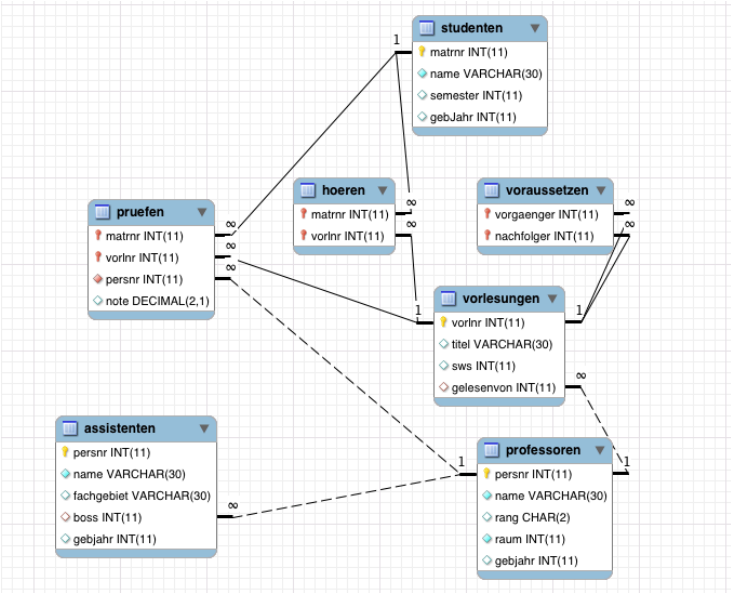
\includegraphics[width=1\textwidth]{./pictures/SQL-DB_ER_Diagramm_UNI-DB.png}
  \caption{ER-Diagramm zur Uni-DB \cite{Kaufmann2016_S1}}
  \label{fig:uni-db}
\end{figure}
 Um mit den NoSQL Datenbanken Erfahrung zu sammeln, wird dieses Schema in die NoSQL Datenbank MongoDB überführt.
Die MongoDB ist eine dokumentorientierte Datenbank und  wird aus folgenden
Gründen für dieses Projekt verwendet:
\begin{itemize}
  \item Geeignet um unser Problem zu lösen.
  \item Wird in der Praxis eingesetzt
  \item Gute Dokumentation
  \item Kostenfrei
  \item Untstützung durch Forenuser
  \item Erste Erfahrung vorhanden
\end{itemize}
Die Aufgabe besteht darin, ein vorgegeben SQL-Query so in MongoDB operationen
abzubilden, dass die MonogDB Abfrage das selbe Resultat ergibt wie das folgende 
SQL-Query
\begin{lstlisting}
select ProfessorName, AnzahlStudenten, SummeSWS 
from ( 
	select p.Name as ProfessorName, count(s.MatrNr) 
	as AnzahlStudenten 
		from Professoren p 
		join Vorlesungen v on v.gelesenVon = p.PersNr
		join hoeren h on h.VorlNr = v.VorlNr 
		join Studenten s on s.MatrNr = h.MatrNr 
		group by p.Name 
	) A 
join 
( 
	select p.Name as ProfessorName,  sum(SWS) 
	as summeSWS 
	from Professoren p 
	join Vorlesungen v on v.gelesenVon = p.PersNr 
	group by p.Name 
) B using(ProfessorName)
\end{lstlisting}